\documentclass[1p]{elsarticle_modified}
%\bibliographystyle{elsarticle-num}

%\usepackage[colorlinks]{hyperref}
%\usepackage{abbrmath_seonhwa} %\Abb, \Ascr, \Acal ,\Abf, \Afrak
\usepackage{amsfonts}
\usepackage{amssymb}
\usepackage{amsmath}
\usepackage{amsthm}
\usepackage{scalefnt}
\usepackage{amsbsy}
\usepackage{kotex}
\usepackage{caption}
\usepackage{subfig}
\usepackage{color}
\usepackage{graphicx}
\usepackage{xcolor} %% white, black, red, green, blue, cyan, magenta, yellow
\usepackage{float}
\usepackage{setspace}
\usepackage{hyperref}

\usepackage{tikz}
\usetikzlibrary{arrows}

\usepackage{multirow}
\usepackage{array} % fixed length table
\usepackage{hhline}

%%%%%%%%%%%%%%%%%%%%%
\makeatletter
\renewcommand*\env@matrix[1][\arraystretch]{%
	\edef\arraystretch{#1}%
	\hskip -\arraycolsep
	\let\@ifnextchar\new@ifnextchar
	\array{*\c@MaxMatrixCols c}}
\makeatother %https://tex.stackexchange.com/questions/14071/how-can-i-increase-the-line-spacing-in-a-matrix
%%%%%%%%%%%%%%%

\usepackage[normalem]{ulem}

\newcommand{\msout}[1]{\ifmmode\text{\sout{\ensuremath{#1}}}\else\sout{#1}\fi}
%SOURCE: \msout is \stkout macro in https://tex.stackexchange.com/questions/20609/strikeout-in-math-mode

\newcommand{\cancel}[1]{
	\ifmmode
	{\color{red}\msout{#1}}
	\else
	{\color{red}\sout{#1}}
	\fi
}

\newcommand{\add}[1]{
	{\color{blue}\uwave{#1}}
}

\newcommand{\replace}[2]{
	\ifmmode
	{\color{red}\msout{#1}}{\color{blue}\uwave{#2}}
	\else
	{\color{red}\sout{#1}}{\color{blue}\uwave{#2}}
	\fi
}

\newcommand{\Sol}{\mathcal{S}} %segment
\newcommand{\D}{D} %diagram
\newcommand{\A}{\mathcal{A}} %arc


%%%%%%%%%%%%%%%%%%%%%%%%%%%%%5 test

\def\sl{\operatorname{\textup{SL}}(2,\Cbb)}
\def\psl{\operatorname{\textup{PSL}}(2,\Cbb)}
\def\quan{\mkern 1mu \triangleright \mkern 1mu}

\theoremstyle{definition}
\newtheorem{thm}{Theorem}[section]
\newtheorem{prop}[thm]{Proposition}
\newtheorem{lem}[thm]{Lemma}
\newtheorem{ques}[thm]{Question}
\newtheorem{cor}[thm]{Corollary}
\newtheorem{defn}[thm]{Definition}
\newtheorem{exam}[thm]{Example}
\newtheorem{rmk}[thm]{Remark}
\newtheorem{alg}[thm]{Algorithm}

\newcommand{\I}{\sqrt{-1}}
\begin{document}

%\begin{frontmatter}
%
%\title{Boundary parabolic representations of knots up to 8 crossings}
%
%%% Group authors per affiliation:
%\author{Yunhi Cho} 
%\address{Department of Mathematics, University of Seoul, Seoul, Korea}
%\ead{yhcho@uos.ac.kr}
%
%
%\author{Seonhwa Kim} %\fnref{s_kim}}
%\address{Center for Geometry and Physics, Institute for Basic Science, Pohang, 37673, Korea}
%\ead{ryeona17@ibs.re.kr}
%
%\author{Hyuk Kim}
%\address{Department of Mathematical Sciences, Seoul National University, Seoul 08826, Korea}
%\ead{hyukkim@snu.ac.kr}
%
%\author{Seokbeom Yoon}
%\address{Department of Mathematical Sciences, Seoul National University, Seoul, 08826,  Korea}
%\ead{sbyoon15@snu.ac.kr}
%
%\begin{abstract}
%We find all boundary parabolic representation of knots up to 8 crossings.
%
%\end{abstract}
%\begin{keyword}
%    \MSC[2010] 57M25 
%\end{keyword}
%
%\end{frontmatter}

%\linenumbers
%\tableofcontents
%
\newcommand\colored[1]{\textcolor{white}{\rule[-0.35ex]{0.8em}{1.4ex}}\kern-0.8em\color{red} #1}%
%\newcommand\colored[1]{\textcolor{white}{ #1}\kern-2.17ex	\textcolor{white}{ #1}\kern-1.81ex	\textcolor{white}{ #1}\kern-2.15ex\color{red}#1	}

{\Large $\underline{12a_{0461}~(K12a_{0461})}$}

\setlength{\tabcolsep}{10pt}
\renewcommand{\arraystretch}{1.6}
\vspace{1cm}\begin{tabular}{m{100pt}>{\centering\arraybackslash}m{274pt}}
\multirow{5}{120pt}{
	\centering
	\includegraphics[width=112pt]{../../../GIT/diagram.site/Diagrams/png/1262_12a_0461.png}\\
\ \ \ A knot diagram\footnotemark}&
\allowdisplaybreaks
\textbf{Linearized knot diagam} \\
\cline{2-2}
 &
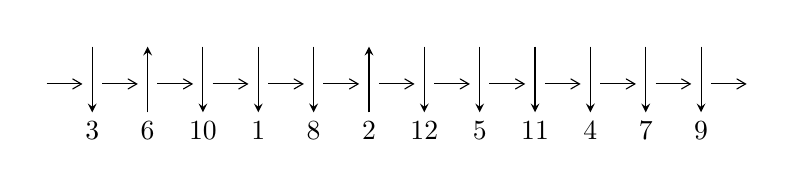
\begin{tikzpicture}[x=20pt, y=17pt]
	% nodes
	\node (C0) at (0, 0) {};
	\node (C1) at (1, 0) {};
	\node (C1U) at (1, +1) {};
	\node (C1D) at (1, -1) {3};

	\node (C2) at (2, 0) {};
	\node (C2U) at (2, +1) {};
	\node (C2D) at (2, -1) {6};

	\node (C3) at (3, 0) {};
	\node (C3U) at (3, +1) {};
	\node (C3D) at (3, -1) {10};

	\node (C4) at (4, 0) {};
	\node (C4U) at (4, +1) {};
	\node (C4D) at (4, -1) {1};

	\node (C5) at (5, 0) {};
	\node (C5U) at (5, +1) {};
	\node (C5D) at (5, -1) {8};

	\node (C6) at (6, 0) {};
	\node (C6U) at (6, +1) {};
	\node (C6D) at (6, -1) {2};

	\node (C7) at (7, 0) {};
	\node (C7U) at (7, +1) {};
	\node (C7D) at (7, -1) {12};

	\node (C8) at (8, 0) {};
	\node (C8U) at (8, +1) {};
	\node (C8D) at (8, -1) {5};

	\node (C9) at (9, 0) {};
	\node (C9U) at (9, +1) {};
	\node (C9D) at (9, -1) {11};

	\node (C10) at (10, 0) {};
	\node (C10U) at (10, +1) {};
	\node (C10D) at (10, -1) {4};

	\node (C11) at (11, 0) {};
	\node (C11U) at (11, +1) {};
	\node (C11D) at (11, -1) {7};

	\node (C12) at (12, 0) {};
	\node (C12U) at (12, +1) {};
	\node (C12D) at (12, -1) {9};
	\node (C13) at (13, 0) {};

	% arrows
	\draw[->,>={angle 60}]
	(C0) edge (C1) (C1) edge (C2) (C2) edge (C3) (C3) edge (C4) (C4) edge (C5) (C5) edge (C6) (C6) edge (C7) (C7) edge (C8) (C8) edge (C9) (C9) edge (C10) (C10) edge (C11) (C11) edge (C12) (C12) edge (C13) ;	\draw[->,>=stealth]
	(C1U) edge (C1D) (C2D) edge (C2U) (C3U) edge (C3D) (C4U) edge (C4D) (C5U) edge (C5D) (C6D) edge (C6U) (C7U) edge (C7D) (C8U) edge (C8D) (C9U) edge (C9D) (C10U) edge (C10D) (C11U) edge (C11D) (C12U) edge (C12D) ;
	\end{tikzpicture} \\
\hhline{~~} \\& 
\textbf{Solving Sequence} \\ \cline{2-2} 
 &
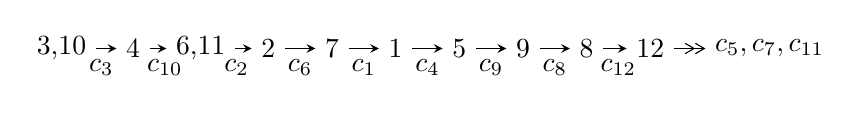
\begin{tikzpicture}[x=23pt, y=7pt]
	% node
	\node (A0) at (-1/8, 0) {3,10};
	\node (A1) at (1, 0) {4};
	\node (A2) at (33/16, 0) {6,11};
	\node (A3) at (25/8, 0) {2};
	\node (A4) at (33/8, 0) {7};
	\node (A5) at (41/8, 0) {1};
	\node (A6) at (49/8, 0) {5};
	\node (A7) at (57/8, 0) {9};
	\node (A8) at (65/8, 0) {8};
	\node (A9) at (73/8, 0) {12};
	\node (C1) at (1/2, -1) {$c_{3}$};
	\node (C2) at (3/2, -1) {$c_{10}$};
	\node (C3) at (21/8, -1) {$c_{2}$};
	\node (C4) at (29/8, -1) {$c_{6}$};
	\node (C5) at (37/8, -1) {$c_{1}$};
	\node (C6) at (45/8, -1) {$c_{4}$};
	\node (C7) at (53/8, -1) {$c_{9}$};
	\node (C8) at (61/8, -1) {$c_{8}$};
	\node (C9) at (69/8, -1) {$c_{12}$};
	\node (A10) at (11, 0) {$c_{5},c_{7},c_{11}$};

	% edge
	\draw[->,>=stealth]	
	(A0) edge (A1) (A1) edge (A2) (A2) edge (A3) (A3) edge (A4) (A4) edge (A5) (A5) edge (A6) (A6) edge (A7) (A7) edge (A8) (A8) edge (A9) ;
	\draw[->>,>={angle 60}]	
	(A9) edge (A10);
\end{tikzpicture} \\ 

\end{tabular} \\

\footnotetext{
The image of knot diagram is generated by the software ``\textbf{Draw programme}" developed by Andrew Bartholomew(\url{http://www.layer8.co.uk/maths/draw/index.htm\#Running-draw}), where we modified some parts for our purpose(\url{https://github.com/CATsTAILs/LinksPainter}).
}\phantom \\ \newline 
\centering \textbf{Ideals for irreducible components\footnotemark of $X_{\text{par}}$} 
 
\begin{align*}
I^u_{1}&=\langle 
-2.78345\times10^{428} u^{153}+4.11856\times10^{427} u^{152}+\cdots+4.56915\times10^{427} b-9.76978\times10^{430},\\
\phantom{I^u_{1}}&\phantom{= \langle  }9.27335\times10^{430} u^{153}-7.70278\times10^{430} u^{152}+\cdots+1.64946\times10^{430} a+5.63983\times10^{433},\\
\phantom{I^u_{1}}&\phantom{= \langle  }u^{154}- u^{153}+\cdots+171 u-361\rangle \\
I^u_{2}&=\langle 
63182 u^{37}+18834 u^{36}+\cdots+9223 b+14567,\;-130140 u^{37}+149794 u^{36}+\cdots+9223 a-397212,\\
\phantom{I^u_{2}}&\phantom{= \langle  }u^{38}-12 u^{36}+\cdots+3 u+1\rangle \\
\\
\end{align*}
\raggedright * 2 irreducible components of $\dim_{\mathbb{C}}=0$, with total 192 representations.\\
\footnotetext{All coefficients of polynomials are rational numbers. But the coefficients are sometimes approximated in decimal forms when there is not enough margin.}
\newpage
\renewcommand{\arraystretch}{1}
\centering \section*{I. $I^u_{1}= \langle -2.78\times10^{428} u^{153}+4.12\times10^{427} u^{152}+\cdots+4.57\times10^{427} b-9.77\times10^{430},\;9.27\times10^{430} u^{153}-7.70\times10^{430} u^{152}+\cdots+1.65\times10^{430} a+5.64\times10^{433},\;u^{154}- u^{153}+\cdots+171 u-361 \rangle$}
\flushleft \textbf{(i) Arc colorings}\\
\begin{tabular}{m{7pt} m{180pt} m{7pt} m{180pt} }
\flushright $a_{3}=$&$\begin{pmatrix}1\\0\end{pmatrix}$ \\
\flushright $a_{10}=$&$\begin{pmatrix}0\\u\end{pmatrix}$ \\
\flushright $a_{4}=$&$\begin{pmatrix}1\\u^2\end{pmatrix}$ \\
\flushright $a_{6}=$&$\begin{pmatrix}-5.62204 u^{153}+4.66987 u^{152}+\cdots-2354.78 u-3419.19\\6.09184 u^{153}-0.901385 u^{152}+\cdots+568.938 u+2138.21\end{pmatrix}$ \\
\flushright $a_{11}=$&$\begin{pmatrix}- u\\- u^3+u\end{pmatrix}$ \\
\flushright $a_{2}=$&$\begin{pmatrix}-5.24596 u^{153}+9.36123 u^{152}+\cdots-4581.17 u-4917.49\\6.95746 u^{153}-3.20412 u^{152}+\cdots+1434.58 u+3079.92\end{pmatrix}$ \\
\flushright $a_{7}=$&$\begin{pmatrix}-5.07748 u^{153}+4.33395 u^{152}+\cdots-2100.13 u-3095.74\\2.24063 u^{153}-1.35986 u^{152}+\cdots+823.755 u+1352.76\end{pmatrix}$ \\
\flushright $a_{1}=$&$\begin{pmatrix}1.71150 u^{153}+6.15711 u^{152}+\cdots-3146.59 u-1837.57\\6.95746 u^{153}-3.20412 u^{152}+\cdots+1434.58 u+3079.92\end{pmatrix}$ \\
\flushright $a_{5}=$&$\begin{pmatrix}-1.38432 u^{153}+1.94270 u^{152}+\cdots-904.514 u-960.807\\-0.598030 u^{153}+0.453949 u^{152}+\cdots-271.071 u-321.745\end{pmatrix}$ \\
\flushright $a_{9}=$&$\begin{pmatrix}u^3\\u^5- u^3+u\end{pmatrix}$ \\
\flushright $a_{8}=$&$\begin{pmatrix}2.43930 u^{153}+2.36182 u^{152}+\cdots-1416.92 u-352.069\\2.30804 u^{153}-0.840085 u^{152}+\cdots+467.621 u+1009.50\end{pmatrix}$ \\
\flushright $a_{12}=$&$\begin{pmatrix}-5.77366 u^{153}+9.18108 u^{152}+\cdots-4535.31 u-5011.51\\6.24262 u^{153}-3.12187 u^{152}+\cdots+1465.57 u+2852.48\end{pmatrix}$\\&\end{tabular}
\flushleft \textbf{(ii) Obstruction class $= -1$}\\~\\
\flushleft \textbf{(iii) Cusp Shapes $= -3.50475 u^{153}+1.30202 u^{152}+\cdots+90.3994 u-1206.07$}\\~\\
\newpage\renewcommand{\arraystretch}{1}
\flushleft \textbf{(iv) u-Polynomials at the component}\newline \\
\begin{tabular}{m{50pt}|m{274pt}}
Crossings & \hspace{64pt}u-Polynomials at each crossing \\
\hline $$\begin{aligned}c_{1}\end{aligned}$$&$\begin{aligned}
&u^{154}+64 u^{153}+\cdots+54112666 u+1857769
\end{aligned}$\\
\hline $$\begin{aligned}c_{2},c_{6}\end{aligned}$$&$\begin{aligned}
&u^{154}-2 u^{153}+\cdots+3074 u+1363
\end{aligned}$\\
\hline $$\begin{aligned}c_{3},c_{10}\end{aligned}$$&$\begin{aligned}
&u^{154}- u^{153}+\cdots+171 u-361
\end{aligned}$\\
\hline $$\begin{aligned}c_{4}\end{aligned}$$&$\begin{aligned}
&u^{154}-6 u^{153}+\cdots+28566941 u+26372777
\end{aligned}$\\
\hline $$\begin{aligned}c_{5},c_{8}\end{aligned}$$&$\begin{aligned}
&u^{154}-3 u^{153}+\cdots+4572 u+4921
\end{aligned}$\\
\hline $$\begin{aligned}c_{7},c_{11}\end{aligned}$$&$\begin{aligned}
&u^{154}+3 u^{153}+\cdots-60545 u-9307
\end{aligned}$\\
\hline $$\begin{aligned}c_{9}\end{aligned}$$&$\begin{aligned}
&u^{154}+71 u^{153}+\cdots+2567071 u+130321
\end{aligned}$\\
\hline $$\begin{aligned}c_{12}\end{aligned}$$&$\begin{aligned}
&u^{154}-3 u^{153}+\cdots-9312 u-521
\end{aligned}$\\
\hline
\end{tabular}\\~\\
\newpage\renewcommand{\arraystretch}{1}
\flushleft \textbf{(v) Riley Polynomials at the component}\newline \\
\begin{tabular}{m{50pt}|m{274pt}}
Crossings & \hspace{64pt}Riley Polynomials at each crossing \\
\hline $$\begin{aligned}c_{1}\end{aligned}$$&$\begin{aligned}
&y^{154}+72 y^{153}+\cdots-893114824048786 y+3451305657361
\end{aligned}$\\
\hline $$\begin{aligned}c_{2},c_{6}\end{aligned}$$&$\begin{aligned}
&y^{154}+64 y^{153}+\cdots+54112666 y+1857769
\end{aligned}$\\
\hline $$\begin{aligned}c_{3},c_{10}\end{aligned}$$&$\begin{aligned}
&y^{154}-71 y^{153}+\cdots-2567071 y+130321
\end{aligned}$\\
\hline $$\begin{aligned}c_{4}\end{aligned}$$&$\begin{aligned}
&y^{154}+46 y^{153}+\cdots+19716884500334309 y+695523366691729
\end{aligned}$\\
\hline $$\begin{aligned}c_{5},c_{8}\end{aligned}$$&$\begin{aligned}
&y^{154}+93 y^{153}+\cdots+417233130 y+24216241
\end{aligned}$\\
\hline $$\begin{aligned}c_{7},c_{11}\end{aligned}$$&$\begin{aligned}
&y^{154}-89 y^{153}+\cdots-3771070879 y+86620249
\end{aligned}$\\
\hline $$\begin{aligned}c_{9}\end{aligned}$$&$\begin{aligned}
&y^{154}+45 y^{153}+\cdots-127131132883 y+16983563041
\end{aligned}$\\
\hline $$\begin{aligned}c_{12}\end{aligned}$$&$\begin{aligned}
&y^{154}+11 y^{153}+\cdots-91631584 y+271441
\end{aligned}$\\
\hline
\end{tabular}\\~\\
\newpage\flushleft \textbf{(vi) Complex Volumes and Cusp Shapes}
$$\begin{array}{c|c|c}  
\text{Solutions to }I^u_{1}& \I (\text{vol} + \sqrt{-1}CS) & \text{Cusp shape}\\
 \hline 
\begin{aligned}
u &= -0.822066 + 0.579429 I \\
a &= -0.444752 + 1.270860 I \\
b &= \phantom{-}1.167560 - 0.604263 I\end{aligned}
 & \phantom{-}4.77078 - 1.29277 I & \phantom{-0.000000 } 0 \\ \hline\begin{aligned}
u &= -0.822066 - 0.579429 I \\
a &= -0.444752 - 1.270860 I \\
b &= \phantom{-}1.167560 + 0.604263 I\end{aligned}
 & \phantom{-}4.77078 + 1.29277 I & \phantom{-0.000000 } 0 \\ \hline\begin{aligned}
u &= \phantom{-}0.894179 + 0.465461 I \\
a &= \phantom{-}2.58293 + 1.18423 I \\
b &= -0.544581 + 0.941019 I\end{aligned}
 & -2.03197 - 3.12428 I & \phantom{-0.000000 } 0 \\ \hline\begin{aligned}
u &= \phantom{-}0.894179 - 0.465461 I \\
a &= \phantom{-}2.58293 - 1.18423 I \\
b &= -0.544581 - 0.941019 I\end{aligned}
 & -2.03197 + 3.12428 I & \phantom{-0.000000 } 0 \\ \hline\begin{aligned}
u &= \phantom{-}0.574939 + 0.805385 I \\
a &= \phantom{-}1.265130 - 0.459295 I \\
b &= -0.826306 + 0.646658 I\end{aligned}
 & \phantom{-}7.65595 + 1.31070 I & \phantom{-0.000000 } 0 \\ \hline\begin{aligned}
u &= \phantom{-}0.574939 - 0.805385 I \\
a &= \phantom{-}1.265130 + 0.459295 I \\
b &= -0.826306 - 0.646658 I\end{aligned}
 & \phantom{-}7.65595 - 1.31070 I & \phantom{-0.000000 } 0 \\ \hline\begin{aligned}
u &= \phantom{-}0.947941 + 0.282051 I \\
a &= \phantom{-}0.30114 - 1.56279 I \\
b &= -0.479556 - 1.140250 I\end{aligned}
 & -3.60832 + 4.35982 I & \phantom{-0.000000 } 0 \\ \hline\begin{aligned}
u &= \phantom{-}0.947941 - 0.282051 I \\
a &= \phantom{-}0.30114 + 1.56279 I \\
b &= -0.479556 + 1.140250 I\end{aligned}
 & -3.60832 - 4.35982 I & \phantom{-0.000000 } 0 \\ \hline\begin{aligned}
u &= \phantom{-}0.987612 + 0.018641 I \\
a &= \phantom{-}0.00318 - 1.91294 I \\
b &= -0.217069 - 0.968326 I\end{aligned}
 & -3.71429 + 2.24347 I & \phantom{-0.000000 } 0 \\ \hline\begin{aligned}
u &= \phantom{-}0.987612 - 0.018641 I \\
a &= \phantom{-}0.00318 + 1.91294 I \\
b &= -0.217069 + 0.968326 I\end{aligned}
 & -3.71429 - 2.24347 I & \phantom{-0.000000 } 0\\
 \hline 
 \end{array}$$\newpage$$\begin{array}{c|c|c}  
\text{Solutions to }I^u_{1}& \I (\text{vol} + \sqrt{-1}CS) & \text{Cusp shape}\\
 \hline 
\begin{aligned}
u &= -0.668369 + 0.726264 I \\
a &= -0.718297 + 0.714281 I \\
b &= \phantom{-}0.551305 - 1.139770 I\end{aligned}
 & \phantom{-}0.97716 - 2.43901 I & \phantom{-0.000000 } 0 \\ \hline\begin{aligned}
u &= -0.668369 - 0.726264 I \\
a &= -0.718297 - 0.714281 I \\
b &= \phantom{-}0.551305 + 1.139770 I\end{aligned}
 & \phantom{-}0.97716 + 2.43901 I & \phantom{-0.000000 } 0 \\ \hline\begin{aligned}
u &= -0.579363 + 0.833528 I \\
a &= -1.173620 + 0.332681 I \\
b &= \phantom{-}0.591151 - 0.942502 I\end{aligned}
 & \phantom{-}1.98078 - 2.74234 I & \phantom{-0.000000 } 0 \\ \hline\begin{aligned}
u &= -0.579363 - 0.833528 I \\
a &= -1.173620 - 0.332681 I \\
b &= \phantom{-}0.591151 + 0.942502 I\end{aligned}
 & \phantom{-}1.98078 + 2.74234 I & \phantom{-0.000000 } 0 \\ \hline\begin{aligned}
u &= \phantom{-}0.871465 + 0.458008 I \\
a &= -1.35338 - 1.13202 I \\
b &= \phantom{-}0.682615 + 0.782945 I\end{aligned}
 & -1.94534 - 0.62809 I & \phantom{-0.000000 } 0 \\ \hline\begin{aligned}
u &= \phantom{-}0.871465 - 0.458008 I \\
a &= -1.35338 + 1.13202 I \\
b &= \phantom{-}0.682615 - 0.782945 I\end{aligned}
 & -1.94534 + 0.62809 I & \phantom{-0.000000 } 0 \\ \hline\begin{aligned}
u &= -0.918836 + 0.451681 I \\
a &= -0.605092 + 0.903934 I \\
b &= -0.175140 + 1.029180 I\end{aligned}
 & -1.93769 + 1.71433 I & \phantom{-0.000000 } 0 \\ \hline\begin{aligned}
u &= -0.918836 - 0.451681 I \\
a &= -0.605092 - 0.903934 I \\
b &= -0.175140 - 1.029180 I\end{aligned}
 & -1.93769 - 1.71433 I & \phantom{-0.000000 } 0 \\ \hline\begin{aligned}
u &= -0.729682 + 0.721684 I \\
a &= \phantom{-}0.486555 - 1.028990 I \\
b &= -0.79150 + 1.18399 I\end{aligned}
 & \phantom{-}2.08567 - 3.75466 I & \phantom{-0.000000 } 0 \\ \hline\begin{aligned}
u &= -0.729682 - 0.721684 I \\
a &= \phantom{-}0.486555 + 1.028990 I \\
b &= -0.79150 - 1.18399 I\end{aligned}
 & \phantom{-}2.08567 + 3.75466 I & \phantom{-0.000000 } 0\\
 \hline 
 \end{array}$$\newpage$$\begin{array}{c|c|c}  
\text{Solutions to }I^u_{1}& \I (\text{vol} + \sqrt{-1}CS) & \text{Cusp shape}\\
 \hline 
\begin{aligned}
u &= -0.520555 + 0.886692 I \\
a &= \phantom{-}1.54611 + 0.12124 I \\
b &= -0.953786 - 0.548158 I\end{aligned}
 & \phantom{-}5.33324 - 7.64609 I & \phantom{-0.000000 } 0 \\ \hline\begin{aligned}
u &= -0.520555 - 0.886692 I \\
a &= \phantom{-}1.54611 - 0.12124 I \\
b &= -0.953786 + 0.548158 I\end{aligned}
 & \phantom{-}5.33324 + 7.64609 I & \phantom{-0.000000 } 0 \\ \hline\begin{aligned}
u &= \phantom{-}0.917644 + 0.474316 I \\
a &= \phantom{-}1.07137 + 1.83095 I \\
b &= -0.568197 - 0.546614 I\end{aligned}
 & -0.18917 - 5.27709 I & \phantom{-0.000000 } 0 \\ \hline\begin{aligned}
u &= \phantom{-}0.917644 - 0.474316 I \\
a &= \phantom{-}1.07137 - 1.83095 I \\
b &= -0.568197 + 0.546614 I\end{aligned}
 & -0.18917 + 5.27709 I & \phantom{-0.000000 } 0 \\ \hline\begin{aligned}
u &= \phantom{-}0.850743 + 0.454824 I \\
a &= -3.54253 - 0.52996 I \\
b &= \phantom{-}0.433739 - 0.796809 I\end{aligned}
 & \phantom{-}0.05968 + 1.50926 I & \phantom{-0.000000 } 0 \\ \hline\begin{aligned}
u &= \phantom{-}0.850743 - 0.454824 I \\
a &= -3.54253 + 0.52996 I \\
b &= \phantom{-}0.433739 + 0.796809 I\end{aligned}
 & \phantom{-}0.05968 - 1.50926 I & \phantom{-0.000000 } 0 \\ \hline\begin{aligned}
u &= -0.497579 + 0.907977 I \\
a &= -1.54017 - 0.19865 I \\
b &= \phantom{-}0.775781 + 0.624816 I\end{aligned}
 & \phantom{-}1.20572 - 1.73714 I & \phantom{-0.000000 } 0 \\ \hline\begin{aligned}
u &= -0.497579 - 0.907977 I \\
a &= -1.54017 + 0.19865 I \\
b &= \phantom{-}0.775781 - 0.624816 I\end{aligned}
 & \phantom{-}1.20572 + 1.73714 I & \phantom{-0.000000 } 0 \\ \hline\begin{aligned}
u &= -0.876837 + 0.560697 I \\
a &= \phantom{-}1.66191 - 0.43835 I \\
b &= -1.21803 - 0.77054 I\end{aligned}
 & \phantom{-}4.60760 + 5.83375 I & \phantom{-0.000000 } 0 \\ \hline\begin{aligned}
u &= -0.876837 - 0.560697 I \\
a &= \phantom{-}1.66191 + 0.43835 I \\
b &= -1.21803 + 0.77054 I\end{aligned}
 & \phantom{-}4.60760 - 5.83375 I & \phantom{-0.000000 } 0\\
 \hline 
 \end{array}$$\newpage$$\begin{array}{c|c|c}  
\text{Solutions to }I^u_{1}& \I (\text{vol} + \sqrt{-1}CS) & \text{Cusp shape}\\
 \hline 
\begin{aligned}
u &= \phantom{-}0.878557 + 0.356936 I \\
a &= -0.899409 + 0.785346 I \\
b &= \phantom{-}0.511909 + 1.111000 I\end{aligned}
 & -3.76126 + 0.86569 I & \phantom{-0.000000 } 0 \\ \hline\begin{aligned}
u &= \phantom{-}0.878557 - 0.356936 I \\
a &= -0.899409 - 0.785346 I \\
b &= \phantom{-}0.511909 - 1.111000 I\end{aligned}
 & -3.76126 - 0.86569 I & \phantom{-0.000000 } 0 \\ \hline\begin{aligned}
u &= -0.892698 + 0.317318 I \\
a &= -0.142050 - 0.305134 I \\
b &= -0.651868 - 0.110332 I\end{aligned}
 & -0.748888 - 0.051632 I & \phantom{-0.000000 } 0 \\ \hline\begin{aligned}
u &= -0.892698 - 0.317318 I \\
a &= -0.142050 + 0.305134 I \\
b &= -0.651868 + 0.110332 I\end{aligned}
 & -0.748888 + 0.051632 I & \phantom{-0.000000 } 0 \\ \hline\begin{aligned}
u &= -0.923163 + 0.505766 I \\
a &= -0.780045 - 0.137098 I \\
b &= \phantom{-}0.759557 + 0.367110 I\end{aligned}
 & -1.46508 + 3.89283 I & \phantom{-0.000000 } 0 \\ \hline\begin{aligned}
u &= -0.923163 - 0.505766 I \\
a &= -0.780045 + 0.137098 I \\
b &= \phantom{-}0.759557 - 0.367110 I\end{aligned}
 & -1.46508 - 3.89283 I & \phantom{-0.000000 } 0 \\ \hline\begin{aligned}
u &= -0.906674 + 0.538347 I \\
a &= \phantom{-}0.95178 - 1.61428 I \\
b &= \phantom{-}0.083826 - 1.026110 I\end{aligned}
 & \phantom{-}0.71731 + 5.70936 I & \phantom{-0.000000 } 0 \\ \hline\begin{aligned}
u &= -0.906674 - 0.538347 I \\
a &= \phantom{-}0.95178 + 1.61428 I \\
b &= \phantom{-}0.083826 + 1.026110 I\end{aligned}
 & \phantom{-}0.71731 - 5.70936 I & \phantom{-0.000000 } 0 \\ \hline\begin{aligned}
u &= \phantom{-}0.820406 + 0.458403 I \\
a &= \phantom{-}0.647027 + 1.181240 I \\
b &= -1.05924 - 1.01980 I\end{aligned}
 & \phantom{-}3.87296 + 2.04708 I & \phantom{-0.000000 } 0 \\ \hline\begin{aligned}
u &= \phantom{-}0.820406 - 0.458403 I \\
a &= \phantom{-}0.647027 - 1.181240 I \\
b &= -1.05924 + 1.01980 I\end{aligned}
 & \phantom{-}3.87296 - 2.04708 I & \phantom{-0.000000 } 0\\
 \hline 
 \end{array}$$\newpage$$\begin{array}{c|c|c}  
\text{Solutions to }I^u_{1}& \I (\text{vol} + \sqrt{-1}CS) & \text{Cusp shape}\\
 \hline 
\begin{aligned}
u &= -0.491837 + 0.939919 I \\
a &= \phantom{-}1.149150 - 0.165391 I \\
b &= -0.665878 + 0.767357 I\end{aligned}
 & \phantom{-}5.03680 + 3.07332 I & \phantom{-0.000000 } 0 \\ \hline\begin{aligned}
u &= -0.491837 - 0.939919 I \\
a &= \phantom{-}1.149150 + 0.165391 I \\
b &= -0.665878 - 0.767357 I\end{aligned}
 & \phantom{-}5.03680 - 3.07332 I & \phantom{-0.000000 } 0 \\ \hline\begin{aligned}
u &= \phantom{-}0.945523 + 0.495565 I \\
a &= -1.99803 - 0.97327 I \\
b &= \phantom{-}0.882851 - 1.066330 I\end{aligned}
 & \phantom{-}3.40570 - 5.90996 I & \phantom{-0.000000 } 0 \\ \hline\begin{aligned}
u &= \phantom{-}0.945523 - 0.495565 I \\
a &= -1.99803 + 0.97327 I \\
b &= \phantom{-}0.882851 + 1.066330 I\end{aligned}
 & \phantom{-}3.40570 + 5.90996 I & \phantom{-0.000000 } 0 \\ \hline\begin{aligned}
u &= \phantom{-}0.770452 + 0.739156 I \\
a &= -1.248880 + 0.251459 I \\
b &= \phantom{-}0.594063 - 0.525342 I\end{aligned}
 & \phantom{-}2.97747 - 1.79063 I & \phantom{-0.000000 } 0 \\ \hline\begin{aligned}
u &= \phantom{-}0.770452 - 0.739156 I \\
a &= -1.248880 - 0.251459 I \\
b &= \phantom{-}0.594063 + 0.525342 I\end{aligned}
 & \phantom{-}2.97747 + 1.79063 I & \phantom{-0.000000 } 0 \\ \hline\begin{aligned}
u &= \phantom{-}0.462193 + 0.966845 I \\
a &= \phantom{-}1.176070 + 0.594409 I \\
b &= -0.713019 - 1.119190 I\end{aligned}
 & \phantom{-}3.5607 + 13.7363 I & \phantom{-0.000000 } 0 \\ \hline\begin{aligned}
u &= \phantom{-}0.462193 - 0.966845 I \\
a &= \phantom{-}1.176070 - 0.594409 I \\
b &= -0.713019 + 1.119190 I\end{aligned}
 & \phantom{-}3.5607 - 13.7363 I & \phantom{-0.000000 } 0 \\ \hline\begin{aligned}
u &= -0.470514 + 0.799319 I \\
a &= \phantom{-}1.355640 - 0.226669 I \\
b &= -0.701764 + 1.026230 I\end{aligned}
 & \phantom{-}6.49583 - 7.02496 I & \phantom{-0.000000 } 0 \\ \hline\begin{aligned}
u &= -0.470514 - 0.799319 I \\
a &= \phantom{-}1.355640 + 0.226669 I \\
b &= -0.701764 - 1.026230 I\end{aligned}
 & \phantom{-}6.49583 + 7.02496 I & \phantom{-0.000000 } 0\\
 \hline 
 \end{array}$$\newpage$$\begin{array}{c|c|c}  
\text{Solutions to }I^u_{1}& \I (\text{vol} + \sqrt{-1}CS) & \text{Cusp shape}\\
 \hline 
\begin{aligned}
u &= \phantom{-}0.815400 + 0.697882 I \\
a &= -1.089590 - 0.840715 I \\
b &= \phantom{-}1.078540 + 0.172318 I\end{aligned}
 & \phantom{-}4.76065 - 2.44822 I & \phantom{-0.000000 } 0 \\ \hline\begin{aligned}
u &= \phantom{-}0.815400 - 0.697882 I \\
a &= -1.089590 + 0.840715 I \\
b &= \phantom{-}1.078540 - 0.172318 I\end{aligned}
 & \phantom{-}4.76065 + 2.44822 I & \phantom{-0.000000 } 0 \\ \hline\begin{aligned}
u &= -0.754448 + 0.536803 I \\
a &= -0.392491 - 0.695246 I \\
b &= \phantom{-}0.146016 - 0.972184 I\end{aligned}
 & \phantom{-}1.17020 - 1.35654 I & \phantom{-0.000000 } 0 \\ \hline\begin{aligned}
u &= -0.754448 - 0.536803 I \\
a &= -0.392491 + 0.695246 I \\
b &= \phantom{-}0.146016 + 0.972184 I\end{aligned}
 & \phantom{-}1.17020 + 1.35654 I & \phantom{-0.000000 } 0 \\ \hline\begin{aligned}
u &= -1.083000 + 0.078736 I \\
a &= \phantom{-}0.174446 - 0.429268 I \\
b &= \phantom{-}0.610702 - 0.769764 I\end{aligned}
 & \phantom{-}1.57089 + 0.38016 I & \phantom{-0.000000 } 0 \\ \hline\begin{aligned}
u &= -1.083000 - 0.078736 I \\
a &= \phantom{-}0.174446 + 0.429268 I \\
b &= \phantom{-}0.610702 + 0.769764 I\end{aligned}
 & \phantom{-}1.57089 - 0.38016 I & \phantom{-0.000000 } 0 \\ \hline\begin{aligned}
u &= \phantom{-}1.022580 + 0.381336 I \\
a &= \phantom{-}0.89246 + 1.66749 I \\
b &= -0.375939 + 1.147050 I\end{aligned}
 & -4.26811 - 3.61828 I & \phantom{-0.000000 } 0 \\ \hline\begin{aligned}
u &= \phantom{-}1.022580 - 0.381336 I \\
a &= \phantom{-}0.89246 - 1.66749 I \\
b &= -0.375939 - 1.147050 I\end{aligned}
 & -4.26811 + 3.61828 I & \phantom{-0.000000 } 0 \\ \hline\begin{aligned}
u &= \phantom{-}0.423073 + 1.008590 I \\
a &= -1.198600 - 0.573364 I \\
b &= \phantom{-}0.673937 + 1.032060 I\end{aligned}
 & -0.02924 + 7.23734 I & \phantom{-0.000000 } 0 \\ \hline\begin{aligned}
u &= \phantom{-}0.423073 - 1.008590 I \\
a &= -1.198600 + 0.573364 I \\
b &= \phantom{-}0.673937 - 1.032060 I\end{aligned}
 & -0.02924 - 7.23734 I & \phantom{-0.000000 } 0\\
 \hline 
 \end{array}$$\newpage$$\begin{array}{c|c|c}  
\text{Solutions to }I^u_{1}& \I (\text{vol} + \sqrt{-1}CS) & \text{Cusp shape}\\
 \hline 
\begin{aligned}
u &= -0.691432 + 0.580549 I \\
a &= \phantom{-}0.46157 - 2.05865 I \\
b &= -0.496029 + 0.785846 I\end{aligned}
 & -1.45978 - 1.10196 I & \phantom{-0.000000 } 0 \\ \hline\begin{aligned}
u &= -0.691432 - 0.580549 I \\
a &= \phantom{-}0.46157 + 2.05865 I \\
b &= -0.496029 - 0.785846 I\end{aligned}
 & -1.45978 + 1.10196 I & \phantom{-0.000000 } 0 \\ \hline\begin{aligned}
u &= \phantom{-}1.093050 + 0.111168 I \\
a &= -0.06711 + 1.46631 I \\
b &= \phantom{-}0.591387 + 0.890936 I\end{aligned}
 & \phantom{-}1.22073 + 5.13744 I & \phantom{-0.000000 } 0 \\ \hline\begin{aligned}
u &= \phantom{-}1.093050 - 0.111168 I \\
a &= -0.06711 - 1.46631 I \\
b &= \phantom{-}0.591387 - 0.890936 I\end{aligned}
 & \phantom{-}1.22073 - 5.13744 I & \phantom{-0.000000 } 0 \\ \hline\begin{aligned}
u &= \phantom{-}0.333598 + 0.828789 I \\
a &= \phantom{-}1.32166 + 0.65256 I \\
b &= -0.786662 - 0.864514 I\end{aligned}
 & \phantom{-}6.44245 + 1.96973 I & \phantom{-0.000000 } 0 \\ \hline\begin{aligned}
u &= \phantom{-}0.333598 - 0.828789 I \\
a &= \phantom{-}1.32166 - 0.65256 I \\
b &= -0.786662 + 0.864514 I\end{aligned}
 & \phantom{-}6.44245 - 1.96973 I & \phantom{-0.000000 } 0 \\ \hline\begin{aligned}
u &= -0.957114 + 0.567759 I \\
a &= -2.30954 - 0.37752 I \\
b &= \phantom{-}0.624720 + 0.894756 I\end{aligned}
 & -2.28055 + 5.68893 I & \phantom{-0.000000 } 0 \\ \hline\begin{aligned}
u &= -0.957114 - 0.567759 I \\
a &= -2.30954 + 0.37752 I \\
b &= \phantom{-}0.624720 - 0.894756 I\end{aligned}
 & -2.28055 - 5.68893 I & \phantom{-0.000000 } 0 \\ \hline\begin{aligned}
u &= -0.415910 + 0.782812 I \\
a &= \phantom{-}1.68218 + 0.31117 I \\
b &= -0.803099 - 0.894750 I\end{aligned}
 & \phantom{-}6.37596 + 3.98356 I & \phantom{-0.000000 } 0 \\ \hline\begin{aligned}
u &= -0.415910 - 0.782812 I \\
a &= \phantom{-}1.68218 - 0.31117 I \\
b &= -0.803099 + 0.894750 I\end{aligned}
 & \phantom{-}6.37596 - 3.98356 I & \phantom{-0.000000 } 0\\
 \hline 
 \end{array}$$\newpage$$\begin{array}{c|c|c}  
\text{Solutions to }I^u_{1}& \I (\text{vol} + \sqrt{-1}CS) & \text{Cusp shape}\\
 \hline 
\begin{aligned}
u &= \phantom{-}0.880709 + 0.702773 I \\
a &= \phantom{-}1.34473 + 0.62320 I \\
b &= -1.070680 + 0.328745 I\end{aligned}
 & \phantom{-}4.57020 - 2.91940 I & \phantom{-0.000000 } 0 \\ \hline\begin{aligned}
u &= \phantom{-}0.880709 - 0.702773 I \\
a &= \phantom{-}1.34473 - 0.62320 I \\
b &= -1.070680 - 0.328745 I\end{aligned}
 & \phantom{-}4.57020 + 2.91940 I & \phantom{-0.000000 } 0 \\ \hline\begin{aligned}
u &= -0.639370 + 0.580078 I \\
a &= -1.55493 + 1.89990 I \\
b &= \phantom{-}0.478663 - 0.967647 I\end{aligned}
 & -0.59318 - 5.24593 I & \phantom{-0.000000 } 0 \\ \hline\begin{aligned}
u &= -0.639370 - 0.580078 I \\
a &= -1.55493 - 1.89990 I \\
b &= \phantom{-}0.478663 + 0.967647 I\end{aligned}
 & -0.59318 + 5.24593 I & \phantom{-0.000000 } 0 \\ \hline\begin{aligned}
u &= -0.991748 + 0.576448 I \\
a &= \phantom{-}2.80809 - 0.23504 I \\
b &= -0.565770 - 1.038220 I\end{aligned}
 & -1.68086 + 9.89233 I & \phantom{-0.000000 } 0 \\ \hline\begin{aligned}
u &= -0.991748 - 0.576448 I \\
a &= \phantom{-}2.80809 + 0.23504 I \\
b &= -0.565770 + 1.038220 I\end{aligned}
 & -1.68086 - 9.89233 I & \phantom{-0.000000 } 0 \\ \hline\begin{aligned}
u &= \phantom{-}1.15171\phantom{ +0.000000I} \\
a &= \phantom{-}0.872755\phantom{ +0.000000I} \\
b &= -0.557285\phantom{ +0.000000I}\end{aligned}
 & -5.43173\phantom{ +0.000000I} & \phantom{-0.000000 } 0 \\ \hline\begin{aligned}
u &= \phantom{-}1.116650 + 0.288251 I \\
a &= -0.551334 + 1.263380 I \\
b &= \phantom{-}0.009952 + 0.320767 I\end{aligned}
 & -1.03953 - 5.47135 I & \phantom{-0.000000 } 0 \\ \hline\begin{aligned}
u &= \phantom{-}1.116650 - 0.288251 I \\
a &= -0.551334 - 1.263380 I \\
b &= \phantom{-}0.009952 - 0.320767 I\end{aligned}
 & -1.03953 + 5.47135 I & \phantom{-0.000000 } 0 \\ \hline\begin{aligned}
u &= \phantom{-}0.842566 + 0.055109 I \\
a &= -0.43533 - 1.72832 I \\
b &= -0.341428 - 1.140430 I\end{aligned}
 & -3.91290 + 2.72338 I & \phantom{-0.000000 } 0\\
 \hline 
 \end{array}$$\newpage$$\begin{array}{c|c|c}  
\text{Solutions to }I^u_{1}& \I (\text{vol} + \sqrt{-1}CS) & \text{Cusp shape}\\
 \hline 
\begin{aligned}
u &= \phantom{-}0.842566 - 0.055109 I \\
a &= -0.43533 + 1.72832 I \\
b &= -0.341428 + 1.140430 I\end{aligned}
 & -3.91290 - 2.72338 I & \phantom{-0.000000 } 0 \\ \hline\begin{aligned}
u &= -1.137590 + 0.235343 I \\
a &= -1.22592 + 0.74369 I \\
b &= \phantom{-}0.167501 + 1.235820 I\end{aligned}
 & -6.05567 - 2.92910 I & \phantom{-0.000000 } 0 \\ \hline\begin{aligned}
u &= -1.137590 - 0.235343 I \\
a &= -1.22592 - 0.74369 I \\
b &= \phantom{-}0.167501 - 1.235820 I\end{aligned}
 & -6.05567 + 2.92910 I & \phantom{-0.000000 } 0 \\ \hline\begin{aligned}
u &= -0.948270 + 0.671042 I \\
a &= -2.00805 + 0.33990 I \\
b &= \phantom{-}0.75652 + 1.30385 I\end{aligned}
 & \phantom{-}1.42242 + 9.08759 I & \phantom{-0.000000 } 0 \\ \hline\begin{aligned}
u &= -0.948270 - 0.671042 I \\
a &= -2.00805 - 0.33990 I \\
b &= \phantom{-}0.75652 - 1.30385 I\end{aligned}
 & \phantom{-}1.42242 - 9.08759 I & \phantom{-0.000000 } 0 \\ \hline\begin{aligned}
u &= \phantom{-}0.948770 + 0.671579 I \\
a &= \phantom{-}0.447129 + 0.925716 I \\
b &= -0.676867 - 0.396420 I\end{aligned}
 & \phantom{-}2.38838 - 3.60572 I & \phantom{-0.000000 } 0 \\ \hline\begin{aligned}
u &= \phantom{-}0.948770 - 0.671579 I \\
a &= \phantom{-}0.447129 - 0.925716 I \\
b &= -0.676867 + 0.396420 I\end{aligned}
 & \phantom{-}2.38838 + 3.60572 I & \phantom{-0.000000 } 0 \\ \hline\begin{aligned}
u &= \phantom{-}1.121990 + 0.364900 I \\
a &= -0.27592 - 1.50625 I \\
b &= \phantom{-}0.447760 - 0.992496 I\end{aligned}
 & -4.54531 - 5.71755 I & \phantom{-0.000000 } 0 \\ \hline\begin{aligned}
u &= \phantom{-}1.121990 - 0.364900 I \\
a &= -0.27592 + 1.50625 I \\
b &= \phantom{-}0.447760 + 0.992496 I\end{aligned}
 & -4.54531 + 5.71755 I & \phantom{-0.000000 } 0 \\ \hline\begin{aligned}
u &= \phantom{-}0.639027 + 1.000420 I \\
a &= \phantom{-}1.242290 - 0.373765 I \\
b &= -0.632031 + 0.914157 I\end{aligned}
 & \phantom{-}4.58793 - 8.11613 I & \phantom{-0.000000 } 0\\
 \hline 
 \end{array}$$\newpage$$\begin{array}{c|c|c}  
\text{Solutions to }I^u_{1}& \I (\text{vol} + \sqrt{-1}CS) & \text{Cusp shape}\\
 \hline 
\begin{aligned}
u &= \phantom{-}0.639027 - 1.000420 I \\
a &= \phantom{-}1.242290 + 0.373765 I \\
b &= -0.632031 - 0.914157 I\end{aligned}
 & \phantom{-}4.58793 + 8.11613 I & \phantom{-0.000000 } 0 \\ \hline\begin{aligned}
u &= \phantom{-}1.055660 + 0.555609 I \\
a &= \phantom{-}0.986123 + 0.387552 I \\
b &= -0.05146 + 1.46074 I\end{aligned}
 & -4.01170 - 10.05950 I & \phantom{-0.000000 } 0 \\ \hline\begin{aligned}
u &= \phantom{-}1.055660 - 0.555609 I \\
a &= \phantom{-}0.986123 - 0.387552 I \\
b &= -0.05146 - 1.46074 I\end{aligned}
 & -4.01170 + 10.05950 I & \phantom{-0.000000 } 0 \\ \hline\begin{aligned}
u &= -0.993474 + 0.666991 I \\
a &= \phantom{-}2.02429 - 0.50756 I \\
b &= -0.533965 - 1.230380 I\end{aligned}
 & \phantom{-}0.00033 + 7.78187 I & \phantom{-0.000000 } 0 \\ \hline\begin{aligned}
u &= -0.993474 - 0.666991 I \\
a &= \phantom{-}2.02429 + 0.50756 I \\
b &= -0.533965 + 1.230380 I\end{aligned}
 & \phantom{-}0.00033 - 7.78187 I & \phantom{-0.000000 } 0 \\ \hline\begin{aligned}
u &= \phantom{-}0.807859 + 0.884061 I \\
a &= -1.293630 + 0.452149 I \\
b &= \phantom{-}0.498444 - 0.759435 I\end{aligned}
 & \phantom{-}2.71484 - 1.73531 I & \phantom{-0.000000 } 0 \\ \hline\begin{aligned}
u &= \phantom{-}0.807859 - 0.884061 I \\
a &= -1.293630 - 0.452149 I \\
b &= \phantom{-}0.498444 + 0.759435 I\end{aligned}
 & \phantom{-}2.71484 + 1.73531 I & \phantom{-0.000000 } 0 \\ \hline\begin{aligned}
u &= -0.706766 + 0.354686 I \\
a &= -0.282796 - 0.622551 I \\
b &= -0.524063 + 0.052177 I\end{aligned}
 & -0.798629 + 0.012049 I & \phantom{-0.000000 } 0 \\ \hline\begin{aligned}
u &= -0.706766 - 0.354686 I \\
a &= -0.282796 + 0.622551 I \\
b &= -0.524063 - 0.052177 I\end{aligned}
 & -0.798629 - 0.012049 I & \phantom{-0.000000 } 0 \\ \hline\begin{aligned}
u &= -1.110330 + 0.484386 I \\
a &= -1.112330 + 0.462518 I \\
b &= -0.294361 + 1.037930 I\end{aligned}
 & -3.47695 + 3.46248 I & \phantom{-0.000000 } 0\\
 \hline 
 \end{array}$$\newpage$$\begin{array}{c|c|c}  
\text{Solutions to }I^u_{1}& \I (\text{vol} + \sqrt{-1}CS) & \text{Cusp shape}\\
 \hline 
\begin{aligned}
u &= -1.110330 - 0.484386 I \\
a &= -1.112330 - 0.462518 I \\
b &= -0.294361 - 1.037930 I\end{aligned}
 & -3.47695 - 3.46248 I & \phantom{-0.000000 } 0 \\ \hline\begin{aligned}
u &= \phantom{-}1.211880 + 0.061782 I \\
a &= -0.476042 + 0.600916 I \\
b &= \phantom{-}0.671000 + 0.365578 I\end{aligned}
 & -1.23772 - 5.74341 I & \phantom{-0.000000 } 0 \\ \hline\begin{aligned}
u &= \phantom{-}1.211880 - 0.061782 I \\
a &= -0.476042 - 0.600916 I \\
b &= \phantom{-}0.671000 - 0.365578 I\end{aligned}
 & -1.23772 + 5.74341 I & \phantom{-0.000000 } 0 \\ \hline\begin{aligned}
u &= \phantom{-}0.106543 + 0.761246 I \\
a &= -0.792451 + 0.559262 I \\
b &= \phantom{-}0.013347 - 1.023550 I\end{aligned}
 & -4.27716 + 1.18904 I & \phantom{-0.000000 } 0 \\ \hline\begin{aligned}
u &= \phantom{-}0.106543 - 0.761246 I \\
a &= -0.792451 - 0.559262 I \\
b &= \phantom{-}0.013347 + 1.023550 I\end{aligned}
 & -4.27716 - 1.18904 I & \phantom{-0.000000 } 0 \\ \hline\begin{aligned}
u &= \phantom{-}0.913187 + 0.827058 I \\
a &= \phantom{-}0.333766 + 0.974109 I \\
b &= -0.321105 - 0.731793 I\end{aligned}
 & \phantom{-}2.41371 - 4.51701 I & \phantom{-0.000000 } 0 \\ \hline\begin{aligned}
u &= \phantom{-}0.913187 - 0.827058 I \\
a &= \phantom{-}0.333766 - 0.974109 I \\
b &= -0.321105 + 0.731793 I\end{aligned}
 & \phantom{-}2.41371 + 4.51701 I & \phantom{-0.000000 } 0 \\ \hline\begin{aligned}
u &= \phantom{-}1.122340 + 0.517563 I \\
a &= -0.585144 - 0.582633 I \\
b &= \phantom{-}0.005654 - 1.207420 I\end{aligned}
 & -7.07290 - 5.73501 I & \phantom{-0.000000 } 0 \\ \hline\begin{aligned}
u &= \phantom{-}1.122340 - 0.517563 I \\
a &= -0.585144 + 0.582633 I \\
b &= \phantom{-}0.005654 + 1.207420 I\end{aligned}
 & -7.07290 + 5.73501 I & \phantom{-0.000000 } 0 \\ \hline\begin{aligned}
u &= -1.142660 + 0.480684 I \\
a &= \phantom{-}0.991446 - 0.372542 I \\
b &= \phantom{-}0.407802 - 0.786236 I\end{aligned}
 & -3.76575 + 2.18592 I & \phantom{-0.000000 } 0\\
 \hline 
 \end{array}$$\newpage$$\begin{array}{c|c|c}  
\text{Solutions to }I^u_{1}& \I (\text{vol} + \sqrt{-1}CS) & \text{Cusp shape}\\
 \hline 
\begin{aligned}
u &= -1.142660 - 0.480684 I \\
a &= \phantom{-}0.991446 + 0.372542 I \\
b &= \phantom{-}0.407802 + 0.786236 I\end{aligned}
 & -3.76575 - 2.18592 I & \phantom{-0.000000 } 0 \\ \hline\begin{aligned}
u &= \phantom{-}1.048440 + 0.669478 I \\
a &= -0.157000 - 1.014550 I \\
b &= \phantom{-}0.820539 + 0.548469 I\end{aligned}
 & \phantom{-}6.23300 - 6.84752 I & \phantom{-0.000000 } 0 \\ \hline\begin{aligned}
u &= \phantom{-}1.048440 - 0.669478 I \\
a &= -0.157000 + 1.014550 I \\
b &= \phantom{-}0.820539 - 0.548469 I\end{aligned}
 & \phantom{-}6.23300 + 6.84752 I & \phantom{-0.000000 } 0 \\ \hline\begin{aligned}
u &= -1.057340 + 0.665573 I \\
a &= \phantom{-}1.97801 - 0.79727 I \\
b &= -0.562818 - 1.051300 I\end{aligned}
 & \phantom{-}0.51473 + 8.33328 I & \phantom{-0.000000 } 0 \\ \hline\begin{aligned}
u &= -1.057340 - 0.665573 I \\
a &= \phantom{-}1.97801 + 0.79727 I \\
b &= -0.562818 + 1.051300 I\end{aligned}
 & \phantom{-}0.51473 - 8.33328 I & \phantom{-0.000000 } 0 \\ \hline\begin{aligned}
u &= -1.095860 + 0.627858 I \\
a &= -1.97338 + 1.14086 I \\
b &= \phantom{-}0.658073 + 1.076560 I\end{aligned}
 & \phantom{-}4.62438 + 12.39440 I & \phantom{-0.000000 } 0 \\ \hline\begin{aligned}
u &= -1.095860 - 0.627858 I \\
a &= -1.97338 - 1.14086 I \\
b &= \phantom{-}0.658073 - 1.076560 I\end{aligned}
 & \phantom{-}4.62438 - 12.39440 I & \phantom{-0.000000 } 0 \\ \hline\begin{aligned}
u &= -0.140721 + 0.720089 I \\
a &= \phantom{-}0.182316 + 0.104872 I \\
b &= -0.558431 - 0.851273 I\end{aligned}
 & -0.87087 + 2.23864 I & \phantom{-0.000000 } 0 \\ \hline\begin{aligned}
u &= -0.140721 - 0.720089 I \\
a &= \phantom{-}0.182316 - 0.104872 I \\
b &= -0.558431 + 0.851273 I\end{aligned}
 & -0.87087 - 2.23864 I & \phantom{-0.000000 } 0 \\ \hline\begin{aligned}
u &= -1.102930 + 0.679166 I \\
a &= -0.562620 + 0.951998 I \\
b &= \phantom{-}1.035360 - 0.490369 I\end{aligned}
 & \phantom{-}3.55762 + 13.43040 I & \phantom{-0.000000 } 0\\
 \hline 
 \end{array}$$\newpage$$\begin{array}{c|c|c}  
\text{Solutions to }I^u_{1}& \I (\text{vol} + \sqrt{-1}CS) & \text{Cusp shape}\\
 \hline 
\begin{aligned}
u &= -1.102930 - 0.679166 I \\
a &= -0.562620 - 0.951998 I \\
b &= \phantom{-}1.035360 + 0.490369 I\end{aligned}
 & \phantom{-}3.55762 - 13.43040 I & \phantom{-0.000000 } 0 \\ \hline\begin{aligned}
u &= -1.112230 + 0.676396 I \\
a &= \phantom{-}0.589980 - 0.830670 I \\
b &= -0.876411 + 0.545244 I\end{aligned}
 & -0.66666 + 7.55235 I & \phantom{-0.000000 } 0 \\ \hline\begin{aligned}
u &= -1.112230 - 0.676396 I \\
a &= \phantom{-}0.589980 + 0.830670 I \\
b &= -0.876411 - 0.545244 I\end{aligned}
 & -0.66666 - 7.55235 I & \phantom{-0.000000 } 0 \\ \hline\begin{aligned}
u &= -1.151800 + 0.621427 I \\
a &= -0.354074 + 0.613260 I \\
b &= \phantom{-}0.822266 - 0.822898 I\end{aligned}
 & \phantom{-}4.15465 + 1.33498 I & \phantom{-0.000000 } 0 \\ \hline\begin{aligned}
u &= -1.151800 - 0.621427 I \\
a &= -0.354074 - 0.613260 I \\
b &= \phantom{-}0.822266 + 0.822898 I\end{aligned}
 & \phantom{-}4.15465 - 1.33498 I & \phantom{-0.000000 } 0 \\ \hline\begin{aligned}
u &= -1.275870 + 0.297568 I \\
a &= \phantom{-}1.008550 - 0.654374 I \\
b &= -0.245337 - 1.054360 I\end{aligned}
 & -8.61445 + 2.72790 I & \phantom{-0.000000 } 0 \\ \hline\begin{aligned}
u &= -1.275870 - 0.297568 I \\
a &= \phantom{-}1.008550 + 0.654374 I \\
b &= -0.245337 + 1.054360 I\end{aligned}
 & -8.61445 - 2.72790 I & \phantom{-0.000000 } 0 \\ \hline\begin{aligned}
u &= -0.228727 + 0.640057 I \\
a &= -0.314354 - 0.294683 I \\
b &= \phantom{-}0.371470 + 1.033300 I\end{aligned}
 & -0.966729 + 0.859390 I & -5.92499 + 0. I\phantom{ +0.000000I} \\ \hline\begin{aligned}
u &= -0.228727 - 0.640057 I \\
a &= -0.314354 + 0.294683 I \\
b &= \phantom{-}0.371470 - 1.033300 I\end{aligned}
 & -0.966729 - 0.859390 I & -5.92499 + 0. I\phantom{ +0.000000I} \\ \hline\begin{aligned}
u &= -1.134690 + 0.716778 I \\
a &= -1.57546 + 0.75755 I \\
b &= \phantom{-}0.568922 + 0.878250 I\end{aligned}
 & \phantom{-}3.09471 + 2.98427 I & \phantom{-0.000000 } 0\\
 \hline 
 \end{array}$$\newpage$$\begin{array}{c|c|c}  
\text{Solutions to }I^u_{1}& \I (\text{vol} + \sqrt{-1}CS) & \text{Cusp shape}\\
 \hline 
\begin{aligned}
u &= -1.134690 - 0.716778 I \\
a &= -1.57546 - 0.75755 I \\
b &= \phantom{-}0.568922 - 0.878250 I\end{aligned}
 & \phantom{-}3.09471 - 2.98427 I & \phantom{-0.000000 } 0 \\ \hline\begin{aligned}
u &= \phantom{-}1.155860 + 0.686217 I \\
a &= -1.91337 - 0.66981 I \\
b &= \phantom{-}0.718805 - 1.172310 I\end{aligned}
 & \phantom{-}1.4255 - 19.7547 I & \phantom{-0.000000 } 0 \\ \hline\begin{aligned}
u &= \phantom{-}1.155860 - 0.686217 I \\
a &= -1.91337 + 0.66981 I \\
b &= \phantom{-}0.718805 + 1.172310 I\end{aligned}
 & \phantom{-}1.4255 + 19.7547 I & \phantom{-0.000000 } 0 \\ \hline\begin{aligned}
u &= \phantom{-}1.207910 + 0.591732 I \\
a &= -1.61200 - 0.68765 I \\
b &= \phantom{-}0.769951 - 0.938293 I\end{aligned}
 & \phantom{-}3.78528 - 7.29732 I & \phantom{-0.000000 } 0 \\ \hline\begin{aligned}
u &= \phantom{-}1.207910 - 0.591732 I \\
a &= -1.61200 + 0.68765 I \\
b &= \phantom{-}0.769951 + 0.938293 I\end{aligned}
 & \phantom{-}3.78528 + 7.29732 I & \phantom{-0.000000 } 0 \\ \hline\begin{aligned}
u &= -1.352950 + 0.028199 I \\
a &= -0.380214 - 0.665078 I \\
b &= \phantom{-}0.598993 - 1.083700 I\end{aligned}
 & -3.19698 - 10.70540 I & \phantom{-0.000000 } 0 \\ \hline\begin{aligned}
u &= -1.352950 - 0.028199 I \\
a &= -0.380214 + 0.665078 I \\
b &= \phantom{-}0.598993 + 1.083700 I\end{aligned}
 & -3.19698 + 10.70540 I & \phantom{-0.000000 } 0 \\ \hline\begin{aligned}
u &= \phantom{-}1.177610 + 0.689514 I \\
a &= \phantom{-}1.84293 + 0.57964 I \\
b &= -0.689134 + 1.096760 I\end{aligned}
 & -2.34666 - 13.36180 I & \phantom{-0.000000 } 0 \\ \hline\begin{aligned}
u &= \phantom{-}1.177610 - 0.689514 I \\
a &= \phantom{-}1.84293 - 0.57964 I \\
b &= -0.689134 - 1.096760 I\end{aligned}
 & -2.34666 + 13.36180 I & \phantom{-0.000000 } 0 \\ \hline\begin{aligned}
u &= \phantom{-}1.085870 + 0.835827 I \\
a &= -0.274618 - 0.628927 I \\
b &= \phantom{-}0.554690 + 0.833924 I\end{aligned}
 & \phantom{-}3.24985 + 1.50408 I & \phantom{-0.000000 } 0\\
 \hline 
 \end{array}$$\newpage$$\begin{array}{c|c|c}  
\text{Solutions to }I^u_{1}& \I (\text{vol} + \sqrt{-1}CS) & \text{Cusp shape}\\
 \hline 
\begin{aligned}
u &= \phantom{-}1.085870 - 0.835827 I \\
a &= -0.274618 + 0.628927 I \\
b &= \phantom{-}0.554690 - 0.833924 I\end{aligned}
 & \phantom{-}3.24985 - 1.50408 I & \phantom{-0.000000 } 0 \\ \hline\begin{aligned}
u &= \phantom{-}0.267156 + 0.504152 I \\
a &= \phantom{-}1.28364 - 0.90605 I \\
b &= \phantom{-}0.163501 + 1.252410 I\end{aligned}
 & -2.12105 + 5.62580 I & -8.69169 - 6.13312 I \\ \hline\begin{aligned}
u &= \phantom{-}0.267156 - 0.504152 I \\
a &= \phantom{-}1.28364 + 0.90605 I \\
b &= \phantom{-}0.163501 - 1.252410 I\end{aligned}
 & -2.12105 - 5.62580 I & -8.69169 + 6.13312 I \\ \hline\begin{aligned}
u &= \phantom{-}0.522745 + 0.193253 I \\
a &= \phantom{-}1.71293 + 0.63012 I \\
b &= \phantom{-}0.326924 + 1.280390 I\end{aligned}
 & -2.07926 + 5.70484 I & -8.22383 - 7.39573 I \\ \hline\begin{aligned}
u &= \phantom{-}0.522745 - 0.193253 I \\
a &= \phantom{-}1.71293 - 0.63012 I \\
b &= \phantom{-}0.326924 - 1.280390 I\end{aligned}
 & -2.07926 - 5.70484 I & -8.22383 + 7.39573 I \\ \hline\begin{aligned}
u &= -0.534086\phantom{ +0.000000I} \\
a &= -0.703155\phantom{ +0.000000I} \\
b &= -0.362371\phantom{ +0.000000I}\end{aligned}
 & -0.932967\phantom{ +0.000000I} & -10.1800\phantom{ +0.000000I} \\ \hline\begin{aligned}
u &= \phantom{-}1.47986 + 0.05680 I \\
a &= \phantom{-}0.858827 + 0.664018 I \\
b &= -0.533518 + 0.707425 I\end{aligned}
 & -5.87293 - 1.10773 I & \phantom{-0.000000 } 0 \\ \hline\begin{aligned}
u &= \phantom{-}1.47986 - 0.05680 I \\
a &= \phantom{-}0.858827 - 0.664018 I \\
b &= -0.533518 - 0.707425 I\end{aligned}
 & -5.87293 + 1.10773 I & \phantom{-0.000000 } 0 \\ \hline\begin{aligned}
u &= -1.48687 + 0.13620 I \\
a &= \phantom{-}0.476101 + 0.355357 I \\
b &= -0.562080 + 0.984677 I\end{aligned}
 & -6.81024 - 3.33209 I & \phantom{-0.000000 } 0 \\ \hline\begin{aligned}
u &= -1.48687 - 0.13620 I \\
a &= \phantom{-}0.476101 - 0.355357 I \\
b &= -0.562080 - 0.984677 I\end{aligned}
 & -6.81024 + 3.33209 I & \phantom{-0.000000 } 0\\
 \hline 
 \end{array}$$\newpage$$\begin{array}{c|c|c}  
\text{Solutions to }I^u_{1}& \I (\text{vol} + \sqrt{-1}CS) & \text{Cusp shape}\\
 \hline 
\begin{aligned}
u &= \phantom{-}0.055894 + 0.485909 I \\
a &= -0.270436 + 1.037490 I \\
b &= \phantom{-}0.612930 + 0.064066 I\end{aligned}
 & \phantom{-}1.80576 + 2.53513 I & -2.13143 - 3.97247 I \\ \hline\begin{aligned}
u &= \phantom{-}0.055894 - 0.485909 I \\
a &= -0.270436 - 1.037490 I \\
b &= \phantom{-}0.612930 - 0.064066 I\end{aligned}
 & \phantom{-}1.80576 - 2.53513 I & -2.13143 + 3.97247 I \\ \hline\begin{aligned}
u &= -0.176421 + 0.374536 I \\
a &= -1.151760 + 0.139094 I \\
b &= \phantom{-}0.288238 + 0.794600 I\end{aligned}
 & -0.452145 + 1.312550 I & -4.74769 - 4.89976 I \\ \hline\begin{aligned}
u &= -0.176421 - 0.374536 I \\
a &= -1.151760 - 0.139094 I \\
b &= \phantom{-}0.288238 - 0.794600 I\end{aligned}
 & -0.452145 - 1.312550 I & -4.74769 + 4.89976 I\\
 \hline 
 \end{array}$$\newpage\newpage\renewcommand{\arraystretch}{1}
\centering \section*{II. $I^u_{2}= \langle 63182 u^{37}+18834 u^{36}+\cdots+9223 b+14567,\;-1.30\times10^{5} u^{37}+1.50\times10^{5} u^{36}+\cdots+9223 a-3.97\times10^{5},\;u^{38}-12 u^{36}+\cdots+3 u+1 \rangle$}
\flushleft \textbf{(i) Arc colorings}\\
\begin{tabular}{m{7pt} m{180pt} m{7pt} m{180pt} }
\flushright $a_{3}=$&$\begin{pmatrix}1\\0\end{pmatrix}$ \\
\flushright $a_{10}=$&$\begin{pmatrix}0\\u\end{pmatrix}$ \\
\flushright $a_{4}=$&$\begin{pmatrix}1\\u^2\end{pmatrix}$ \\
\flushright $a_{6}=$&$\begin{pmatrix}14.1104 u^{37}-16.2414 u^{36}+\cdots+92.0837 u+43.0675\\-6.85048 u^{37}-2.04207 u^{36}+\cdots+20.1664 u-1.57942\end{pmatrix}$ \\
\flushright $a_{11}=$&$\begin{pmatrix}- u\\- u^3+u\end{pmatrix}$ \\
\flushright $a_{2}=$&$\begin{pmatrix}-2.94123 u^{37}+0.382305 u^{36}+\cdots-3.13618 u-0.270519\\3.14876 u^{37}+0.790632 u^{36}+\cdots-4.18974 u+2.62149\end{pmatrix}$ \\
\flushright $a_{7}=$&$\begin{pmatrix}11.4728 u^{37}-3.77263 u^{36}+\cdots+30.8969 u+9.83259\\-1.89602 u^{37}+4.91998 u^{36}+\cdots-19.2041 u-12.5248\end{pmatrix}$ \\
\flushright $a_{1}=$&$\begin{pmatrix}0.207525 u^{37}+1.17294 u^{36}+\cdots-7.32592 u+2.35097\\3.14876 u^{37}+0.790632 u^{36}+\cdots-4.18974 u+2.62149\end{pmatrix}$ \\
\flushright $a_{5}=$&$\begin{pmatrix}6.50038 u^{37}-3.41635 u^{36}+\cdots+60.6781 u+26.3995\\-0.171311 u^{37}+0.523908 u^{36}+\cdots+3.46341 u-3.79443\end{pmatrix}$ \\
\flushright $a_{9}=$&$\begin{pmatrix}u^3\\u^5- u^3+u\end{pmatrix}$ \\
\flushright $a_{8}=$&$\begin{pmatrix}27.6979 u^{37}-5.58506 u^{36}+\cdots-11.7576 u+16.9625\\5.27366 u^{37}+0.894720 u^{36}+\cdots-23.8593 u-9.72840\end{pmatrix}$ \\
\flushright $a_{12}=$&$\begin{pmatrix}-0.792475 u^{37}+1.17294 u^{36}+\cdots-7.32592 u+2.35097\\3.14876 u^{37}+0.790632 u^{36}+\cdots-3.18974 u+2.62149\end{pmatrix}$\\&\end{tabular}
\flushleft \textbf{(ii) Obstruction class $= 1$}\\~\\
\flushleft \textbf{(iii) Cusp Shapes $= -\frac{125590}{9223} u^{37}+\frac{9092}{9223} u^{36}+\cdots-\frac{355732}{9223} u-\frac{476456}{9223}$}\\~\\
\newpage\renewcommand{\arraystretch}{1}
\flushleft \textbf{(iv) u-Polynomials at the component}\newline \\
\begin{tabular}{m{50pt}|m{274pt}}
Crossings & \hspace{64pt}u-Polynomials at each crossing \\
\hline $$\begin{aligned}c_{1}\end{aligned}$$&$\begin{aligned}
&u^{38}-19 u^{37}+\cdots-24 u+1
\end{aligned}$\\
\hline $$\begin{aligned}c_{2}\end{aligned}$$&$\begin{aligned}
&u^{38}- u^{37}+\cdots+12 u^2+1
\end{aligned}$\\
\hline $$\begin{aligned}c_{3}\end{aligned}$$&$\begin{aligned}
&u^{38}-12 u^{36}+\cdots+3 u+1
\end{aligned}$\\
\hline $$\begin{aligned}c_{4}\end{aligned}$$&$\begin{aligned}
&u^{38}+u^{37}+\cdots-5 u+1
\end{aligned}$\\
\hline $$\begin{aligned}c_{5}\end{aligned}$$&$\begin{aligned}
&u^{38}-4 u^{37}+\cdots-2 u+1
\end{aligned}$\\
\hline $$\begin{aligned}c_{6}\end{aligned}$$&$\begin{aligned}
&u^{38}+u^{37}+\cdots+12 u^2+1
\end{aligned}$\\
\hline $$\begin{aligned}c_{7}\end{aligned}$$&$\begin{aligned}
&u^{38}+2 u^{37}+\cdots+u+1
\end{aligned}$\\
\hline $$\begin{aligned}c_{8}\end{aligned}$$&$\begin{aligned}
&u^{38}+4 u^{37}+\cdots+2 u+1
\end{aligned}$\\
\hline $$\begin{aligned}c_{9}\end{aligned}$$&$\begin{aligned}
&u^{38}-24 u^{37}+\cdots-21 u+1
\end{aligned}$\\
\hline $$\begin{aligned}c_{10}\end{aligned}$$&$\begin{aligned}
&u^{38}-12 u^{36}+\cdots-3 u+1
\end{aligned}$\\
\hline $$\begin{aligned}c_{11}\end{aligned}$$&$\begin{aligned}
&u^{38}-2 u^{37}+\cdots- u+1
\end{aligned}$\\
\hline $$\begin{aligned}c_{12}\end{aligned}$$&$\begin{aligned}
&u^{38}+6 u^{37}+\cdots-10 u+1
\end{aligned}$\\
\hline
\end{tabular}\\~\\
\newpage\renewcommand{\arraystretch}{1}
\flushleft \textbf{(v) Riley Polynomials at the component}\newline \\
\begin{tabular}{m{50pt}|m{274pt}}
Crossings & \hspace{64pt}Riley Polynomials at each crossing \\
\hline $$\begin{aligned}c_{1}\end{aligned}$$&$\begin{aligned}
&y^{38}+19 y^{37}+\cdots+12 y+1
\end{aligned}$\\
\hline $$\begin{aligned}c_{2},c_{6}\end{aligned}$$&$\begin{aligned}
&y^{38}+19 y^{37}+\cdots+24 y+1
\end{aligned}$\\
\hline $$\begin{aligned}c_{3},c_{10}\end{aligned}$$&$\begin{aligned}
&y^{38}-24 y^{37}+\cdots-21 y+1
\end{aligned}$\\
\hline $$\begin{aligned}c_{4}\end{aligned}$$&$\begin{aligned}
&y^{38}+5 y^{37}+\cdots+19 y+1
\end{aligned}$\\
\hline $$\begin{aligned}c_{5},c_{8}\end{aligned}$$&$\begin{aligned}
&y^{38}+20 y^{37}+\cdots+36 y+1
\end{aligned}$\\
\hline $$\begin{aligned}c_{7},c_{11}\end{aligned}$$&$\begin{aligned}
&y^{38}-30 y^{37}+\cdots-33 y+1
\end{aligned}$\\
\hline $$\begin{aligned}c_{9}\end{aligned}$$&$\begin{aligned}
&y^{38}-28 y^{36}+\cdots-21 y+1
\end{aligned}$\\
\hline $$\begin{aligned}c_{12}\end{aligned}$$&$\begin{aligned}
&y^{38}-6 y^{37}+\cdots-42 y+1
\end{aligned}$\\
\hline
\end{tabular}\\~\\
\newpage\flushleft \textbf{(vi) Complex Volumes and Cusp Shapes}
$$\begin{array}{c|c|c}  
\text{Solutions to }I^u_{2}& \I (\text{vol} + \sqrt{-1}CS) & \text{Cusp shape}\\
 \hline 
\begin{aligned}
u &= \phantom{-}0.991867 + 0.293008 I \\
a &= \phantom{-}0.088290 + 0.480131 I \\
b &= -0.341002 + 1.107610 I\end{aligned}
 & -3.11280 - 7.15236 I & -11.2847 + 9.0430 I \\ \hline\begin{aligned}
u &= \phantom{-}0.991867 - 0.293008 I \\
a &= \phantom{-}0.088290 - 0.480131 I \\
b &= -0.341002 - 1.107610 I\end{aligned}
 & -3.11280 + 7.15236 I & -11.2847 - 9.0430 I \\ \hline\begin{aligned}
u &= \phantom{-}0.732096 + 0.626334 I \\
a &= -1.67555 - 0.49709 I \\
b &= \phantom{-}1.036790 - 0.718459 I\end{aligned}
 & \phantom{-}4.91223 - 4.80789 I & -3.00260 + 3.79185 I \\ \hline\begin{aligned}
u &= \phantom{-}0.732096 - 0.626334 I \\
a &= -1.67555 + 0.49709 I \\
b &= \phantom{-}1.036790 + 0.718459 I\end{aligned}
 & \phantom{-}4.91223 + 4.80789 I & -3.00260 - 3.79185 I \\ \hline\begin{aligned}
u &= -0.748299 + 0.742347 I \\
a &= \phantom{-}0.711126 - 0.885387 I \\
b &= -0.582385 + 1.100190 I\end{aligned}
 & \phantom{-}0.62663 - 3.36395 I & -9.20426 + 4.94587 I \\ \hline\begin{aligned}
u &= -0.748299 - 0.742347 I \\
a &= \phantom{-}0.711126 + 0.885387 I \\
b &= -0.582385 - 1.100190 I\end{aligned}
 & \phantom{-}0.62663 + 3.36395 I & -9.20426 - 4.94587 I \\ \hline\begin{aligned}
u &= \phantom{-}0.839841 + 0.293635 I \\
a &= \phantom{-}1.06189 + 1.73136 I \\
b &= \phantom{-}0.358348 + 1.192970 I\end{aligned}
 & -2.56301 + 4.67338 I & -10.21931 - 3.08914 I \\ \hline\begin{aligned}
u &= \phantom{-}0.839841 - 0.293635 I \\
a &= \phantom{-}1.06189 - 1.73136 I \\
b &= \phantom{-}0.358348 - 1.192970 I\end{aligned}
 & -2.56301 - 4.67338 I & -10.21931 + 3.08914 I \\ \hline\begin{aligned}
u &= -1.075490 + 0.300288 I \\
a &= -0.14453 + 2.09621 I \\
b &= -0.205733 + 0.743835 I\end{aligned}
 & -1.56441 + 4.82049 I & -14.5664 - 2.6540 I \\ \hline\begin{aligned}
u &= -1.075490 - 0.300288 I \\
a &= -0.14453 - 2.09621 I \\
b &= -0.205733 - 0.743835 I\end{aligned}
 & -1.56441 - 4.82049 I & -14.5664 + 2.6540 I\\
 \hline 
 \end{array}$$\newpage$$\begin{array}{c|c|c}  
\text{Solutions to }I^u_{2}& \I (\text{vol} + \sqrt{-1}CS) & \text{Cusp shape}\\
 \hline 
\begin{aligned}
u &= \phantom{-}0.854395 + 0.767581 I \\
a &= -0.682159 - 1.047860 I \\
b &= \phantom{-}0.281279 + 0.516482 I\end{aligned}
 & \phantom{-}2.84860 - 4.96095 I & -2.01482 + 8.52252 I \\ \hline\begin{aligned}
u &= \phantom{-}0.854395 - 0.767581 I \\
a &= -0.682159 + 1.047860 I \\
b &= \phantom{-}0.281279 - 0.516482 I\end{aligned}
 & \phantom{-}2.84860 + 4.96095 I & -2.01482 - 8.52252 I \\ \hline\begin{aligned}
u &= \phantom{-}1.075450 + 0.417540 I \\
a &= -0.16590 - 1.61326 I \\
b &= \phantom{-}0.290951 - 1.004320 I\end{aligned}
 & -5.01160 - 4.75346 I & -15.3943 + 3.4825 I \\ \hline\begin{aligned}
u &= \phantom{-}1.075450 - 0.417540 I \\
a &= -0.16590 + 1.61326 I \\
b &= \phantom{-}0.290951 + 1.004320 I\end{aligned}
 & -5.01160 + 4.75346 I & -15.3943 - 3.4825 I \\ \hline\begin{aligned}
u &= -0.943617 + 0.669429 I \\
a &= -2.23938 + 0.34377 I \\
b &= \phantom{-}0.552077 + 1.202540 I\end{aligned}
 & \phantom{-}0.03099 + 8.74330 I & -8.91907 - 10.84509 I \\ \hline\begin{aligned}
u &= -0.943617 - 0.669429 I \\
a &= -2.23938 - 0.34377 I \\
b &= \phantom{-}0.552077 - 1.202540 I\end{aligned}
 & \phantom{-}0.03099 - 8.74330 I & -8.91907 + 10.84509 I \\ \hline\begin{aligned}
u &= -0.686929 + 0.483998 I \\
a &= -0.62902 + 1.50618 I \\
b &= \phantom{-}1.027270 - 0.964833 I\end{aligned}
 & \phantom{-}4.24690 - 2.58803 I & -2.22978 + 7.46639 I \\ \hline\begin{aligned}
u &= -0.686929 - 0.483998 I \\
a &= -0.62902 - 1.50618 I \\
b &= \phantom{-}1.027270 + 0.964833 I\end{aligned}
 & \phantom{-}4.24690 + 2.58803 I & -2.22978 - 7.46639 I \\ \hline\begin{aligned}
u &= \phantom{-}0.895125 + 0.796856 I \\
a &= \phantom{-}1.375030 - 0.178060 I \\
b &= -0.393497 + 0.543408 I\end{aligned}
 & \phantom{-}2.72633 - 0.91164 I & -6.33413 - 3.56727 I \\ \hline\begin{aligned}
u &= \phantom{-}0.895125 - 0.796856 I \\
a &= \phantom{-}1.375030 + 0.178060 I \\
b &= -0.393497 - 0.543408 I\end{aligned}
 & \phantom{-}2.72633 + 0.91164 I & -6.33413 + 3.56727 I\\
 \hline 
 \end{array}$$\newpage$$\begin{array}{c|c|c}  
\text{Solutions to }I^u_{2}& \I (\text{vol} + \sqrt{-1}CS) & \text{Cusp shape}\\
 \hline 
\begin{aligned}
u &= -1.068930 + 0.542210 I \\
a &= \phantom{-}1.82807 - 0.68045 I \\
b &= -0.868761 - 1.014880 I\end{aligned}
 & \phantom{-}2.90354 + 6.79041 I & -10.77255 - 7.64968 I \\ \hline\begin{aligned}
u &= -1.068930 - 0.542210 I \\
a &= \phantom{-}1.82807 + 0.68045 I \\
b &= -0.868761 + 1.014880 I\end{aligned}
 & \phantom{-}2.90354 - 6.79041 I & -10.77255 + 7.64968 I \\ \hline\begin{aligned}
u &= -1.104200 + 0.482481 I \\
a &= \phantom{-}1.41930 - 0.31782 I \\
b &= \phantom{-}0.256385 - 0.879117 I\end{aligned}
 & -4.49779 + 2.49920 I & -17.5876 - 2.3366 I \\ \hline\begin{aligned}
u &= -1.104200 - 0.482481 I \\
a &= \phantom{-}1.41930 + 0.31782 I \\
b &= \phantom{-}0.256385 + 0.879117 I\end{aligned}
 & -4.49779 - 2.49920 I & -17.5876 + 2.3366 I \\ \hline\begin{aligned}
u &= \phantom{-}1.008320 + 0.675509 I \\
a &= \phantom{-}0.585134 + 0.669247 I \\
b &= -0.868472 - 0.629081 I\end{aligned}
 & \phantom{-}4.02350 - 0.28612 I & -5.68627 + 0. I\phantom{ +0.000000I} \\ \hline\begin{aligned}
u &= \phantom{-}1.008320 - 0.675509 I \\
a &= \phantom{-}0.585134 - 0.669247 I \\
b &= -0.868472 + 0.629081 I\end{aligned}
 & \phantom{-}4.02350 + 0.28612 I & -5.68627 + 0. I\phantom{ +0.000000I} \\ \hline\begin{aligned}
u &= -0.750582 + 0.224491 I \\
a &= \phantom{-}2.48091 + 0.03823 I \\
b &= \phantom{-}0.130888 + 0.676207 I\end{aligned}
 & -0.27120 - 2.53382 I & -11.47078 + 5.16775 I \\ \hline\begin{aligned}
u &= -0.750582 - 0.224491 I \\
a &= \phantom{-}2.48091 - 0.03823 I \\
b &= \phantom{-}0.130888 - 0.676207 I\end{aligned}
 & -0.27120 + 2.53382 I & -11.47078 - 5.16775 I \\ \hline\begin{aligned}
u &= \phantom{-}0.697328 + 0.208539 I \\
a &= \phantom{-}0.39805 - 2.20775 I \\
b &= -0.387499 - 1.077190 I\end{aligned}
 & -3.23941 + 1.85645 I & -10.13432 - 0.54316 I \\ \hline\begin{aligned}
u &= \phantom{-}0.697328 - 0.208539 I \\
a &= \phantom{-}0.39805 + 2.20775 I \\
b &= -0.387499 + 1.077190 I\end{aligned}
 & -3.23941 - 1.85645 I & -10.13432 + 0.54316 I\\
 \hline 
 \end{array}$$\newpage$$\begin{array}{c|c|c}  
\text{Solutions to }I^u_{2}& \I (\text{vol} + \sqrt{-1}CS) & \text{Cusp shape}\\
 \hline 
\begin{aligned}
u &= -0.188715 + 0.580646 I \\
a &= -0.315921 + 0.452263 I \\
b &= -0.386853 - 0.873194 I\end{aligned}
 & -2.02228 + 1.65299 I & -11.55346 - 2.70930 I \\ \hline\begin{aligned}
u &= -0.188715 - 0.580646 I \\
a &= -0.315921 - 0.452263 I \\
b &= -0.386853 + 0.873194 I\end{aligned}
 & -2.02228 - 1.65299 I & -11.55346 + 2.70930 I \\ \hline\begin{aligned}
u &= \phantom{-}1.400070 + 0.020540 I \\
a &= -0.511954 + 0.412824 I \\
b &= \phantom{-}0.492777 + 0.991292 I\end{aligned}
 & -6.99257 + 2.83923 I & \phantom{-0.000000 } 0 \\ \hline\begin{aligned}
u &= \phantom{-}1.400070 - 0.020540 I \\
a &= -0.511954 - 0.412824 I \\
b &= \phantom{-}0.492777 - 0.991292 I\end{aligned}
 & -6.99257 - 2.83923 I & \phantom{-0.000000 } 0 \\ \hline\begin{aligned}
u &= -1.43299 + 0.02985 I \\
a &= -0.910284 + 0.776573 I \\
b &= \phantom{-}0.494779 + 0.709703 I\end{aligned}
 & -6.02241 + 1.20982 I & \phantom{-0.000000 } 0 \\ \hline\begin{aligned}
u &= -1.43299 - 0.02985 I \\
a &= -0.910284 - 0.776573 I \\
b &= \phantom{-}0.494779 - 0.709703 I\end{aligned}
 & -6.02241 - 1.20982 I & \phantom{-0.000000 } 0 \\ \hline\begin{aligned}
u &= -0.494736 + 0.110162 I \\
a &= -1.17311 + 1.64447 I \\
b &= -0.387344 - 0.683093 I\end{aligned}
 & -1.82565 + 1.31247 I & -12.61929 - 3.30037 I \\ \hline\begin{aligned}
u &= -0.494736 - 0.110162 I \\
a &= -1.17311 - 1.64447 I \\
b &= -0.387344 + 0.683093 I\end{aligned}
 & -1.82565 - 1.31247 I & -12.61929 + 3.30037 I\\
 \hline 
 \end{array}$$\newpage
\newpage\renewcommand{\arraystretch}{1}
\centering \section*{ III. u-Polynomials}
\begin{tabular}{m{50pt}|m{274pt}}
Crossings & \hspace{64pt}u-Polynomials at each crossing \\
\hline $$\begin{aligned}c_{1}\end{aligned}$$&$\begin{aligned}
&(u^{38}-19 u^{37}+\cdots-24 u+1)\\
&\cdot(u^{154}+64 u^{153}+\cdots+54112666 u+1857769)
\end{aligned}$\\
\hline $$\begin{aligned}c_{2}\end{aligned}$$&$\begin{aligned}
&(u^{38}- u^{37}+\cdots+12 u^2+1)(u^{154}-2 u^{153}+\cdots+3074 u+1363)
\end{aligned}$\\
\hline $$\begin{aligned}c_{3}\end{aligned}$$&$\begin{aligned}
&(u^{38}-12 u^{36}+\cdots+3 u+1)(u^{154}- u^{153}+\cdots+171 u-361)
\end{aligned}$\\
\hline $$\begin{aligned}c_{4}\end{aligned}$$&$\begin{aligned}
&(u^{38}+u^{37}+\cdots-5 u+1)\\
&\cdot(u^{154}-6 u^{153}+\cdots+28566941 u+26372777)
\end{aligned}$\\
\hline $$\begin{aligned}c_{5}\end{aligned}$$&$\begin{aligned}
&(u^{38}-4 u^{37}+\cdots-2 u+1)(u^{154}-3 u^{153}+\cdots+4572 u+4921)
\end{aligned}$\\
\hline $$\begin{aligned}c_{6}\end{aligned}$$&$\begin{aligned}
&(u^{38}+u^{37}+\cdots+12 u^2+1)(u^{154}-2 u^{153}+\cdots+3074 u+1363)
\end{aligned}$\\
\hline $$\begin{aligned}c_{7}\end{aligned}$$&$\begin{aligned}
&(u^{38}+2 u^{37}+\cdots+u+1)(u^{154}+3 u^{153}+\cdots-60545 u-9307)
\end{aligned}$\\
\hline $$\begin{aligned}c_{8}\end{aligned}$$&$\begin{aligned}
&(u^{38}+4 u^{37}+\cdots+2 u+1)(u^{154}-3 u^{153}+\cdots+4572 u+4921)
\end{aligned}$\\
\hline $$\begin{aligned}c_{9}\end{aligned}$$&$\begin{aligned}
&(u^{38}-24 u^{37}+\cdots-21 u+1)\\
&\cdot(u^{154}+71 u^{153}+\cdots+2567071 u+130321)
\end{aligned}$\\
\hline $$\begin{aligned}c_{10}\end{aligned}$$&$\begin{aligned}
&(u^{38}-12 u^{36}+\cdots-3 u+1)(u^{154}- u^{153}+\cdots+171 u-361)
\end{aligned}$\\
\hline $$\begin{aligned}c_{11}\end{aligned}$$&$\begin{aligned}
&(u^{38}-2 u^{37}+\cdots- u+1)(u^{154}+3 u^{153}+\cdots-60545 u-9307)
\end{aligned}$\\
\hline $$\begin{aligned}c_{12}\end{aligned}$$&$\begin{aligned}
&(u^{38}+6 u^{37}+\cdots-10 u+1)(u^{154}-3 u^{153}+\cdots-9312 u-521)
\end{aligned}$\\
\hline
\end{tabular}\newpage\renewcommand{\arraystretch}{1}
\centering \section*{ IV. Riley Polynomials}
\begin{tabular}{m{50pt}|m{274pt}}
Crossings & \hspace{64pt}Riley Polynomials at each crossing \\
\hline $$\begin{aligned}c_{1}\end{aligned}$$&$\begin{aligned}
&(y^{38}+19 y^{37}+\cdots+12 y+1)\\
&\cdot(y^{154}+72 y^{153}+\cdots-893114824048786 y+3451305657361)
\end{aligned}$\\
\hline $$\begin{aligned}c_{2},c_{6}\end{aligned}$$&$\begin{aligned}
&(y^{38}+19 y^{37}+\cdots+24 y+1)\\
&\cdot(y^{154}+64 y^{153}+\cdots+54112666 y+1857769)
\end{aligned}$\\
\hline $$\begin{aligned}c_{3},c_{10}\end{aligned}$$&$\begin{aligned}
&(y^{38}-24 y^{37}+\cdots-21 y+1)\\
&\cdot(y^{154}-71 y^{153}+\cdots-2567071 y+130321)
\end{aligned}$\\
\hline $$\begin{aligned}c_{4}\end{aligned}$$&$\begin{aligned}
&(y^{38}+5 y^{37}+\cdots+19 y+1)\\
&\cdot(y^{154}+46 y^{153}+\cdots+19716884500334309 y+695523366691729)
\end{aligned}$\\
\hline $$\begin{aligned}c_{5},c_{8}\end{aligned}$$&$\begin{aligned}
&(y^{38}+20 y^{37}+\cdots+36 y+1)\\
&\cdot(y^{154}+93 y^{153}+\cdots+417233130 y+24216241)
\end{aligned}$\\
\hline $$\begin{aligned}c_{7},c_{11}\end{aligned}$$&$\begin{aligned}
&(y^{38}-30 y^{37}+\cdots-33 y+1)\\
&\cdot(y^{154}-89 y^{153}+\cdots-3771070879 y+86620249)
\end{aligned}$\\
\hline $$\begin{aligned}c_{9}\end{aligned}$$&$\begin{aligned}
&(y^{38}-28 y^{36}+\cdots-21 y+1)\\
&\cdot(y^{154}+45 y^{153}+\cdots-127131132883 y+16983563041)
\end{aligned}$\\
\hline $$\begin{aligned}c_{12}\end{aligned}$$&$\begin{aligned}
&(y^{38}-6 y^{37}+\cdots-42 y+1)\\
&\cdot(y^{154}+11 y^{153}+\cdots-91631584 y+271441)
\end{aligned}$\\
\hline
\end{tabular}
\vskip 2pc
\end{document}